%%%%%%%%%%%%%%%%%%%%%%%%%%%%%%%%%%%%%%%%%
% Dreuw & Deselaer's Poster
% LaTeX Template
% Version 1.0 (11/04/13)
%
% Created by:
% Philippe Dreuw and Thomas Deselaers
% http://www-i6.informatik.rwth-aachen.de/~dreuw/latexbeamerposter.php
%
% This template has been downloaded from:
% http://www.LaTeXTemplates.com
%
% License:
% CC BY-NC-SA 3.0 (http://creativecommons.org/licenses/by-nc-sa/3.0/)
%
%%%%%%%%%%%%%%%%%%%%%%%%%%%%%%%%%%%%%%%%%

%----------------------------------------------------------------------------------------
%	PACKAGES AND OTHER DOCUMENT CONFIGURATIONS
%----------------------------------------------------------------------------------------

\documentclass[final,hyperref={pdfpagelabels=false}]{beamer}

\usepackage[orientation=portrait,size=a0,scale=1.4]{beamerposter} % Use the beamerposter package for laying out the poster with a portrait orientation and an a0 paper size

\usetheme{I6pd2} % Use the I6pd2 theme supplied with this template

\usepackage[utf8]{inputenc} % enconding utf8
\usepackage[portuguese]{babel} % Portuguese language/hyphenation

\usepackage{amsmath,amsthm,amssymb,latexsym} % For including math equations, theorems, symbols, etc

%\usepackage{times}\usefonttheme{professionalfonts}  % Uncomment to use Times as the main font
%\usefonttheme[onlymath]{serif} % Uncomment to use a Serif font within math environments

\boldmath % Use bold for everything within the math environment

\usepackage{booktabs} % Top and bottom rules for tables

\graphicspath{{figures/}} % Location of the graphics files

\usecaptiontemplate{\small\structure{\insertcaptionname~\insertcaptionnumber: }\insertcaption} % A fix for figure numbering

\usepackage[]{url}
\urlstyle{sf}

%----------------------------------------------------------------------------------------
%	TITLE SECTION 
%----------------------------------------------------------------------------------------

\title{\huge Material Didático sobre Algoritmos Gulosos} % Poster title

\author{Victor de Oliveira Colombo} % Author(s)

\institute{Instituto de Matemática e Estatística da Universidade de São Paulo} % Institution(s)

%----------------------------------------------------------------------------------------
%	FOOTER TEXT
%----------------------------------------------------------------------------------------

\newcommand{\leftfoot}{} % Left footer text

\newcommand{\rightfoot}{} % Right footer text

%----------------------------------------------------------------------------------------

\begin{document}

\addtobeamertemplate{block end}{}{\vspace*{2ex}} % White space under blocks

\begin{frame}[t] % The whole poster is enclosed in one beamer frame

\begin{columns}[t] % The whole poster consists of two major columns, each of which can be subdivided further with another \begin{columns} block - the [t] argument aligns each column's content to the top

\begin{column}{.02\textwidth}\end{column} % Empty spacer column

\begin{column}{.465\textwidth} % The first column

%----------------------------------------------------------------------------------------
%	OBJECTIVES
%----------------------------------------------------------------------------------------

\begin{block}{Objetivos}

\begin{itemize}

\item Apresentar algoritmos gulosos de uma maneira pragmática, a partir de problemas
de competições de programação, como a Maratona de Programação, destoando dos problemas
clássicos que são frequentemente abordados nos livros-texto.

\item Resolver problemas que utilizem algoritmos gulosos aliados a outros tópicos, como Programação Dinâmica, Busca Binária e estruturas de dados.

\item Desenvolver o raciocínio e a intuição por trás das técnicas gulosas, a fim de criar uma ferramenta
sistemática para resolvê-los.

\end{itemize}

\end{block}

%----------------------------------------------------------------------------------------
%	Problema da Partição modificado
%----------------------------------------------------------------------------------------
            
\begin{block}{Problema exemplo: Problema da Partição modificado}
\begin{itemize}

\item É dado um vetor de $n$ números inteiros, $V = \{v_1, v_2, ..., v_n\}$.
\item Queremos encontrar $r = \{r_1, r_2, ..., r_n\}$, com $r_i \in \{-1, 1\}$ para todo $i \in [1, n]$, tal que:
$$\sum_{i = 1}^n v_i*r_i = 0$$
\item Ao contrário do Problema da Partição clássico, que é NP-completo, há a restrição de que $1 \leq v_i \leq i$ para todo $i \in [1, n].$
\end{itemize}

\end{block}

%----------------------------------------------------------------------------------------
%	Blog
%----------------------------------------------------------------------------------------

\begin{block}{Desenvolvimento}

\begin{itemize}

\item É fácil ver que se $\sum_{i = 1}^n v_i$ é ímpar, não há solução.
\item Caso contrário, cada partição deve somar:
$$\frac{\sum_{i = 1}^n v_i}{2}$$
\item Ideia: Encaminhar o elemento $v_i$ para a partição mais vazia.
\item \textbf{Não funciona} quando se itera de $1$ a $n$.\\
Contraexemplo: $V = \{1, 2, 3, 4\}$ resulta em partições de somas distintas $4$ e $6$.
\item \textbf{Funciona} quando se itera de $n$ a $1$.
\end{itemize}

\end{block}

%----------------------------------------------------------------------------------------
%	ContestWatcher
%----------------------------------------------------------------------------------------

\begin{block}{Ideias para demonstração}

\begin{itemize}
\item Na iteração $n - i + 1$ do algoritmo, definir a ``folga'' de cada partição, $a_i$ e $b_i$.
\item Mostrar, por contradição, que \underline{alguma} partição terá ``folga'' suficiente em todas as iterações.
\item Utilizar a restrição $1 \leq v_i \leq i$ e quebrar em dois casos: paridade de $a_i$ e $b_i$ são iguais ou diferentes.
\item Montar intervalos de $a_i + b_i$ e notar que suas intersecções são vazias, levando ao absurdo.

\end{itemize}

\end{block}

%----------------------------------------------------------------------------------------
%   ContestWatcher
%----------------------------------------------------------------------------------------

\begin{block}{Corolários e Implementação}

\begin{itemize}

\item $\sum_{i = 1}^n v_i$ é par $\Leftrightarrow$ Há solução.
\item Se existe ``folga'' suficiente nas duas partições, o elemento pode ser encaminhado para \textbf{qualquer} partição (não necessáriamente a menor).
\end{itemize}

\begin{figure}
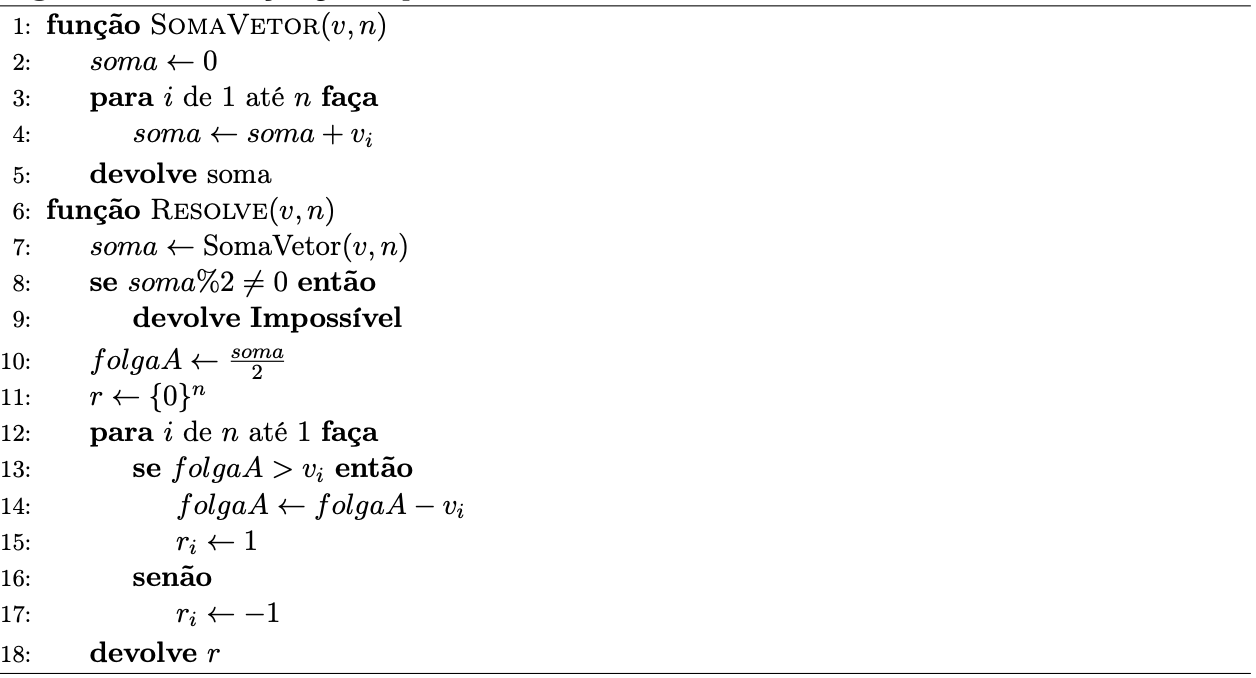
\includegraphics[width=0.8\linewidth]{pseudo.png}
\caption{Pseudocódigo para resolução do Problema da Partição modificado}
\end{figure}

\begin{itemize}
\item Consome tempo $O(n)$ e memória $O(1)$.
\end{itemize}

\end{block}


%----------------------------------------------------------------------------------------

\end{column} % End of the first column

\begin{column}{.03\textwidth}\end{column} % Empty spacer column
 
\begin{column}{.465\textwidth} % The second column

%----------------------------------------------------------------------------------------
%	MaratonIME
%----------------------------------------------------------------------------------------

\begin{block}{Argumento de troca}

\begin{itemize}
\item É muito comum que problemas que aceitam soluções gulosas possuam diversas outras soluções
ótimas.

\item Demonstrações por contradição que assumem a existência de uma solução ótima que
é diferente da solução gulosa são \textbf{insuficientes}.

\item Alternativa: Tomamos uma solução ótima “mais parecida” com a solução gulosa possível.

\item A solução gulosa for ótima, elas coincidirão.

\item Encontrar a contradição o assumindo que as escolhas diferem em algum momento. Tentar
“trocar” a decisão da solução ótima pela solução gulosa e mostramos que tal troca não altera o
resultado.

\end{itemize}
     
\end{block}

%----------------------------------------------------------------------------------------
%	Seletiva Individual
%----------------------------------------------------------------------------------------

\begin{block}{Problema exemplo: Salto do sapo}

Existem pedras $n$ pedras numa reta numérica, em posições distintas $v_1, v_2, ..., v_{n - 1}, v_n$. Dizemos que o sapo pode saltar de uma pedra $v_i$ para outra pedra $v_j$ desde que a distância entre elas seja menor ou igual a $\Delta$. Um sapo está inicialmente na pedra $v_1$. Qual é o menor número de saltos que ele precisa dar para chegar na pedra $v_n$? 

\begin{figure}
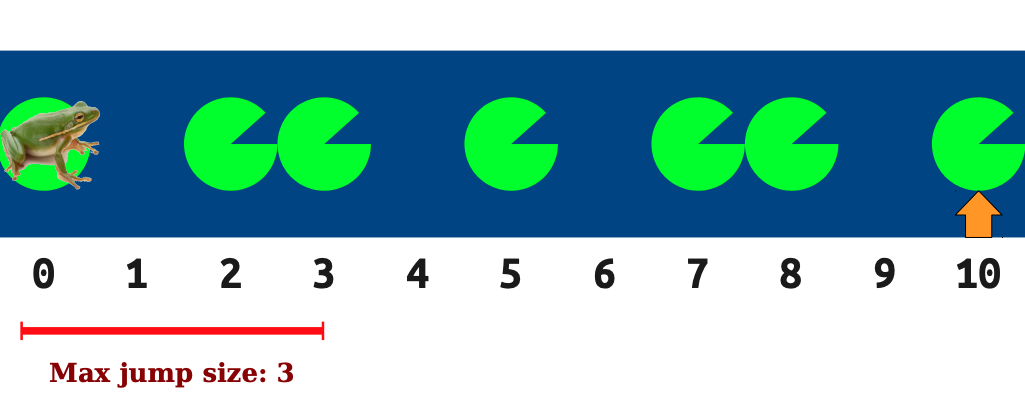
\includegraphics[width=0.8\linewidth]{sapo.png}
\caption{Exemplo para $v = \{0, 2, 3, 5, 7, 8, 10\}$ e $\Delta = 3$.\\
Fonte: https://web.stanford.edu/class/archive/cs/cs161/cs161.1138/lectures/13/Slides13.pdf}
\end{figure}

Algumas soluções para a instância acima são:

\begin{itemize}
    \item $0 \rightarrow 3 \rightarrow 5 \rightarrow 8 \rightarrow 10$
    \item $0 \rightarrow 2 \rightarrow 5 \rightarrow 7 \rightarrow 10$
\end{itemize}

\end{block}

%----------------------------------------------------------------------------------------
% Simulado de Bixes
%----------------------------------------------------------------------------------------

\begin{block}{Desenvolvimento}

\begin{itemize}
    \item Intuitivamente,  nunca vale a pena “voltar”, isto é, escolher um número menor que o escolhido anteriormente, pois isto aumentaria desnecessariamente a sequência, já que poderíamos descartar a escolha anterior e escolher apenas o menor número diretamente.
    \item É intuitivo também que sempre vale a pena dar o maior salto possível, pois não há vantagem de estar numa pedra mais distante do objetivo.
    \item Disso segue um simples algoritmo: a cada iteração, saltar para a pedra mais distante da atual (em direção ao destino) que esteja no alcance do sapo.
\end{itemize}

\end{block}

%----------------------------------------------------------------------------------------
% Simulado de Bixes
%----------------------------------------------------------------------------------------

\begin{block}{Idea de demonstração}

\begin{itemize}
    \item Seja uma sequência de saltos produzida pelo algoritmo guloso $u = \{u_1, u_2, ..., u_k\}$ e uma sequência de saltos ótima $u^* = \{u^*_1, u^*_2, ..., u^*_{k^*}\}$ com maior prefixo de escolhas em comum com $u$. 
    \item Suponha que $u \neq u^*$. Seja $l$ o índice da primeira diferença entre $u$ e $u^*$.
    \item Podemos \textbf{trocar} $u^*_l$ por $u_l$ mantendo a solução ótima válida.
    \item Encontramos assim $\bar{u} = \{u_1, u_2, ..., u_l, u^*_{l + 1}, u^*_{l + 2}, ..., u^*_{k^*}\}$ que é tão bom quanto $u^*$ mas mais com maior prefixo em comum com $u$, contrariando a hipótese.
\end{itemize}

\end{block}

%----------------------------------------------------------------------------------------
%	Veja mais
%----------------------------------------------------------------------------------------

\begin{block}{Veja mais}

Mais problemas e demonstrações completas diponíveis na monografia, acessível em \url{https://linux.ime.usp.br/~colombo/mac0499/}

\end{block}

%----------------------------------------------------------------------------------------

\end{column} % End of the second column

\begin{column}{.015\textwidth}\end{column} % Empty spacer column

\end{columns} % End of all the columns in the poster

\end{frame} % End of the enclosing frame

\end{document}